\chapter{Konzepte}
\label{ch:concept}

\section{Zielsetzung}
\label{sec:zielsetzung}
Wie bereits in Kapitel \ref{ch:intro} beschrieben, dient diese Studienarbeit zur Wissenserweiterung im Bereich der analogen Schaltungstechnik.
Darüber hinaus soll im Zuge dieser Arbeit ein einsetzbarer modularer Synthesizer gebaut werden, der zu elektronischen Klangerzeugung genutzt werden kann. 
Der Synthesizer soll aus verschiedenen Modulen bestehen, welche unabhängig von einander genutzt werden können. 
Der weitere Aufbau wird in Abschnitt \ref{sec:AufbauSynth} genauer beschrieben. 
%Darüber hinaus werden in Abschnitt \ref{sec:AnalogePrinzipien} grundlegende Prinzipien erläutert, die insbesondere bei der elektronischen Klangerzeugung Anwendung finden.


\section{Aufbau eines modularen Synthesizers}
\label{sec:AufbauSynth}
Wie bereits in Abschnitt \ref{sec:zielsetzung} erläutert, besteht ein modularer Synthesizer aus mehreren vereinzelten Modulen. 
Diese Module können mit Kabeln verbunden und somit in Interaktion miteinander gebracht werden. 

Um eine grundlegende Funktion zu ermöglichen, ist ein Basisumfang an Modulen nötig.
Die hierfür nötigen Komponenten oder Module werden im Folgenden aufgelistet und kurz erläutert.

\begin{itemize}
	\item Netzteil:\newline
	Das Netzteil ist elementarer Bestandteil des Synthesizers und stellt die benötigten Spannungslevel zur Versorgung der einzelnen Module bereit.
	Insbesondere für den Einsatz von Operationsverstärkern sind symmetrische Spannungsversorgungen erforderlich.
	
	\item VCO: \newline
	Der VCO (Voltage Controlled Oscillator) ist ein spannungsgesteuerter Oszillator und stellt die Basis bei analogen Synthesizern dar.
	Über eine Steuerspannung kann die Frequenz des erzeugten Signals und somit die Tonhöhe verändert werden. 
	%Verbreitete Signale zur elektronischen Tonerzeugung stellen das Sägezahn- und das Rechtecksignal dar.
	\item VCA: \newline
	Der VCA (Voltage Controlled Amplifier) stellt einen spannungsgesteuerten Verstärker da. 
	Dieser ermöglicht durch Veränderung der Steuerspannung die Beeinflussung der Lautstärke des Signals.
	
	\item ADSR: \newline
	ADSR steht für die vier Phasen einer Hüllkurve: Attack, Decay, Sustain und Release. 
	Eingesetzt werden ADSR-Hüllkurven, um den Verlauf von Lautstärke von Tönen zu steuern. Üblicherweise legt man die Hüllkurve an den Steuereingang eines spannungsgesteuerten Verstärkers (VCA). 
	
	\item VCF: \newline
	Der VCF (Voltage Controlled Filter) ermöglicht durch Veränderung der Steuerspannung die Steuerung des Filterverhaltens.
	Durch Variieren der Eingangsspannung erfolgt die Veränderung der Filtereckfrequenz.
	Die Filterung verschiedener Frequenzanteile beeinflusst den Klang des Signals.
	
	\item Audio Mixer: \newline
	Der Audio Mixer verknüpft verschiedene Signale miteinandern, wodurch neue Signalformen und Klänge generiert werden können.
	
	\item Sequenzer: \newline
	Der Sequenzer erzeugt seriell alternierende Spannungsfolgen, die durch verschiedene Kippschalter und Potentiometer sowohl die einzelnen Spannungspegel als auch die gesamte Geschwindigkeit des Signals variieren. 
	In der Regel werden die Ausgangssignale des Sequenzers zur Ansteuerung weiterer Module – den sogenannten spannungsgesteuerten-Modulen – hergenommen. Neben den Oszillatoren bildet der Sequenzer somit die Basis der Synthesizer-Module.
	
	\item LFO: \newline
	Ein LFO (Low Frequency Oscillator) wird genutzt, um niederfrequente Signale zu erzeugen.
	Typischerweise wird er LFO genutzt, um andere Module anzusteuern.
	
	
%	\item Gehäuse : \newline
%	Um den Synthesizer gut bedienen zu können und um die enthaltenen Komponenten vor schädlichen Einflüssen zu Schützen ist es sinnvoll, 
%	die Module in einem Gehäuse zu verbauen. Dieses besteht üblicherweise aus zwei Schienen mit Anschraubmöglichkeiten, 
%	auf welchen die Frontplatten der einzelnen Module geschraubt werden können.  
\end{itemize}

Um den groben Aufbau und die dahinter liegende Struktur zu verdeutlichen, ist in Abbildung \ref{fig:Produktarchitektur} die Architektur eines modularen Synthesizers aufgezeigt.

\begin{figure}[h]
	\centering
	\setlength{\fboxsep}{1pt} %Abstand der Linien zur Abbildung
	\setlength{\fboxrule}{1pt} %Dicke der Linie
	\fbox{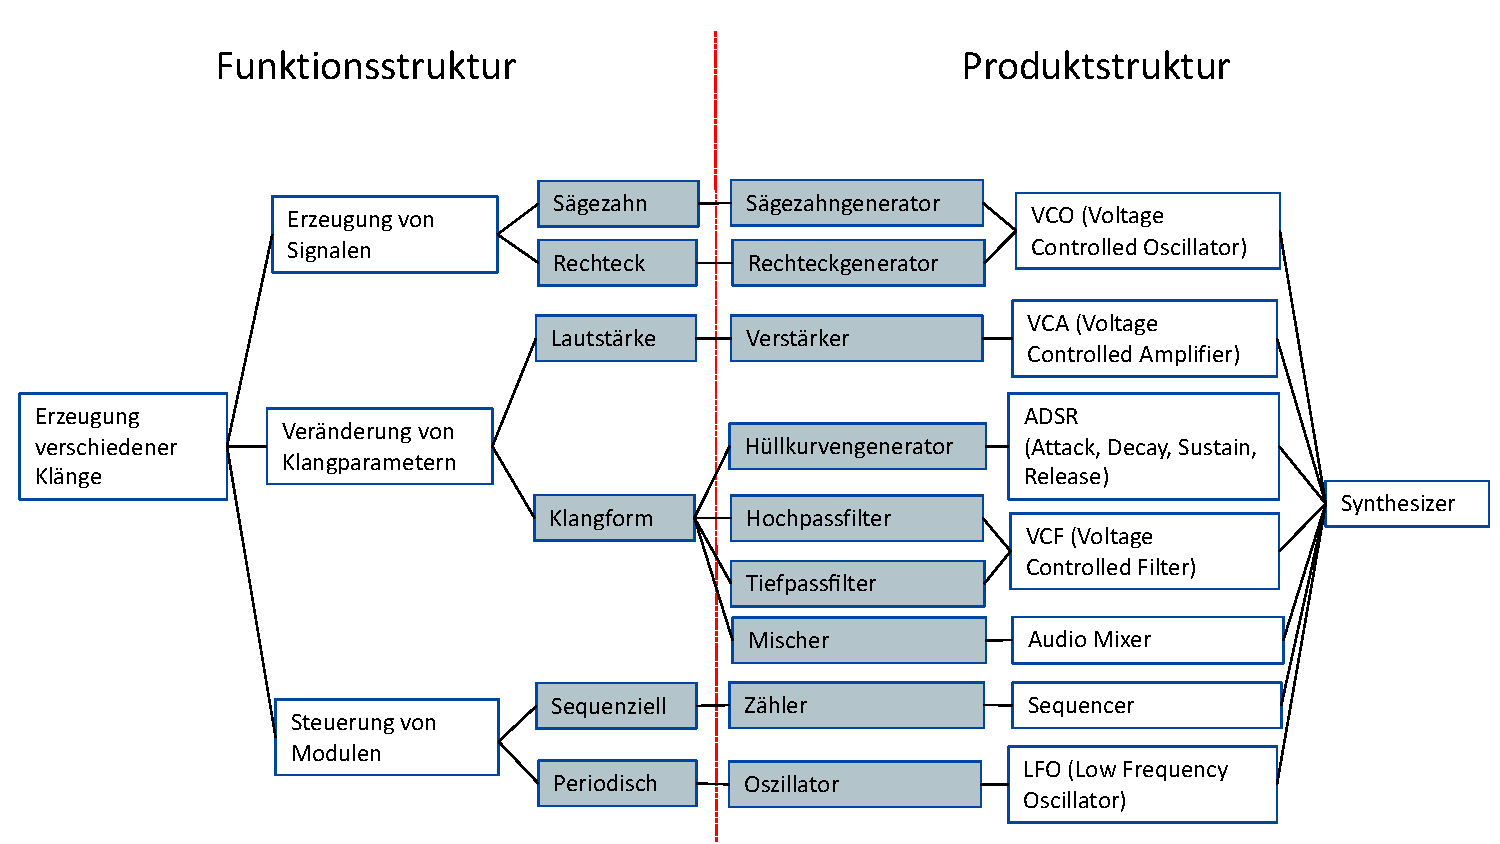
\includegraphics[width=0.8\textwidth]{figures/Produktarchitektur.pdf}}
	\caption{Architektur eines  modularen Synthesizers}
	\label{fig:Produktarchitektur}
\end{figure}


%\newpage
%\section{Grundlegende analoge Prinzipien}
%\label{sec:AnalogePrinzipien}
%
%Exkurs zum Thema Ton/Klang 
%Grundton, Obertöne etc.!




